\documentclass[12pt,a4paper]{article}

\usepackage[utf8]{inputenc}
\usepackage[T1]{fontenc}
\usepackage{amsmath,amssymb,amsthm}
\usepackage{graphicx}
\usepackage{booktabs}
\usepackage{geometry}
\usepackage{setspace}
\usepackage{natbib}
\usepackage{hyperref}
\usepackage{caption}
\usepackage{subcaption}

\geometry{margin=1in}
\onehalfspacing

\hypersetup{
  colorlinks=true,
  linkcolor=blue!60!black,
  citecolor=blue!60!black,
  urlcolor=blue!60!black
}

\newtheorem{proposition}{Proposition}
\newtheorem{definition}{Definition}
\newtheorem{remark}{Remark}

\title{%
  \textbf{Emergent Inequality from Equal Starts:}\\[0.4em]
  Unbiased Wealth Exchange and the Matthew Effect
}

\author{%
  Scott Brodie Forsyth
}

\date{\today}

\begin{document}

% ---------------------------------------------------------------------------
% Epigraph: Matthew 25:29
% ---------------------------------------------------------------------------
\begin{center}
  \textit{``For to all those who have, more will be given, and they will have an abundance;}\\
  \textit{but from those who have nothing, even what they have will be taken away.''}\\[0.6em]
  \textsc{Matthew} 25:29 \citep{matthew2529}
\end{center}

\vspace{1.5em}

\maketitle

\begin{abstract}
  \noindent
  Does inequality require that agents differ in talent, effort, or institutional advantage from the outset?
  This paper argues that it does not.
  In agent-based models of wealth exchange with identical initial endowments and \emph{unbiased} interaction rules---fair coin flips, no preferential flow toward the already-rich---inequality emerges as a generic outcome of stochastic dynamics \citep{dragulescu2000, yakovenko2009}.
  We formalize three such specifications (random fixed transfers, saving-propensity exchange, and yard-sale min-stake losses) and demonstrate the core claim with a Monte Carlo ensemble of $1{,}000$ independent unbiased runs, each beginning at Gini zero and ending with strictly positive dispersion.
  Only after establishing this baseline do we introduce a fourth, \emph{extension} model that operationalizes Merton's Matthew effect: wealth flows toward the richer party with probability $p > \tfrac{1}{2}$ \citep{merton1968, price1976}.
  That bias accelerates concentration but is not necessary for inequality to appear.
  We report Gini coefficients, Lorenz curves, and top wealth shares, with exposition aimed at both specialists and non-specialists.
\end{abstract}

\noindent\textbf{Keywords:} agent-based model; emergent inequality; wealth distribution; unbiased exchange; Matthew effect; cumulative advantage; econophysics

\noindent\textbf{JEL codes:} C63, D31, E17, C15

\vspace{1em}

% ===========================================================================
\section{Introduction}
\label{sec:intro}
% ===========================================================================

A familiar puzzle runs through discussions of inequality: if people start on equal footing, why do outcomes diverge?
One might answer that the rich are favored by institutions, networks, or compounding returns.
That answer points to \emph{cumulative advantage}.
The Gospel of Matthew and Robert K. Merton's \emph{Matthew effect} in science name this force explicitly: resources accrue to those who already hold them \citep{merton1968, matthew2529}.

But cumulative advantage is not the only route to dispersion.
A more basic question comes first: can inequality arise when \emph{nobody} is favored---when every agent starts with the same wealth and every encounter is governed by a symmetric, unbiased rule?
The answer, in the kinetic exchange models studied here, is yes.
Inequality is \emph{emergent}: it is not assumed at $t=0$ but generated by the history of random meetings \citep{dragulescu2000, schelling1971, epstein2006, farmer2013}.

This paper is organized around that ordering.
\textbf{Act I (core).} Models 1--3 use no bias toward the wealthier agent.
Agents meet in pairs; winners and losers are chosen by fair coin flips or by rules that do not tilt toward the rich.
Aggregate wealth is conserved.
Nevertheless, the distribution departs from perfect equality.
We stress-test the claim with $1{,}000$ independent simulations of the minimal unbiased model (Figure~\ref{fig:ensemble}).

\textbf{Act II (extension).} Model 4 adds a small bias $p > \tfrac{1}{2}$ favoring the richer party in each encounter.
This is the Matthew effect as \emph{amplification}: it speeds concentration but is not the existence proof for inequality itself.

The epigraph from Matthew therefore frames the second act, not the first.
The primary scientific contribution is that identical starting points and unbiased exchange suffice to destroy equality.

% ===========================================================================
\section{Conceptual framework}
\label{sec:concepts}
% ===========================================================================

\subsection{Agent-based economic simulation}

An \textbf{agent-based economic simulation} is a computer model in which autonomous agents follow explicit interaction rules.
Macroscopic patterns---here, the wealth distribution---are generated bottom-up rather than imposed \citep{epstein2006, farmer2013}.

\subsection{Emergent inequality}

\textbf{Emergent inequality} means dispersion in outcomes that arises from system dynamics even when initial conditions are symmetric.
All agents begin with $w_i(0) = w_0$.
Any subsequent variance is endogenous.
Crucially, emergent inequality in Act I does \textbf{not} require that richer agents win more often.
Unbiased coin flips are enough.

\subsection{Wealth condensation}

\textbf{Wealth condensation} is the extreme limit in which a vanishing fraction of agents holds a positive share of total wealth \citep{bouchaud2000, ispolatov1998}.
In our simulations, yard-sale and saving-propensity rules (still without rich-agent bias) approach this regime faster than pure random exchange.
Condensation is driven by the \emph{structure} of the bet (multiplicative or min-stake updates), not by naming one agent as inherently superior.

\subsection{The Matthew effect (extension)}

Merton's \emph{Matthew effect} describes cumulative advantage: current stock raises the expected future increment \citep{merton1968, price1976}.
We implement this only in Model~4, where wealth flows to the richer agent with probability $p > \tfrac{1}{2}$.
When $p = \tfrac{1}{2}$, Model~4 collapses to unbiased exchange.
The Matthew effect is therefore an \emph{optional amplifier}, tested comparatively after the unbiased baseline is established.

\begin{remark}[For the non-specialist reader]
  The \textbf{Gini coefficient} summarizes inequality from $0$ (everyone equal) to $1$ (one person holds everything).
  The \textbf{Lorenz curve} plots cumulative wealth against cumulative population; the farther it falls below the diagonal, the greater the inequality \citep{lorenz1905, gini1912}.
\end{remark}

% ===========================================================================
\section{Model}
\label{sec:model}
% ===========================================================================

\subsection{Environment}

Consider $N$ agents $\mathcal{N} = \{1,\ldots,N\}$ in a closed economy.
Each holds wealth $w_i(t) \geq 0$.
Initial endowments are identical:
\begin{equation}
  w_i(0) = w_0 \qquad \forall i \in \mathcal{N}.
  \label{eq:init}
\end{equation}
Wealth is conserved:
\begin{equation}
  \sum_{i=1}^{N} w_i(t) = N w_0 \qquad \forall t.
  \label{eq:conservation}
\end{equation}
Each step, a pair $(i,j)$ is drawn uniformly and an exchange rule updates their wealth.
This is a \emph{kinetic exchange model} \citep{yakovenko2009, lux2008}: production, credit, and taxation are omitted to isolate exchange dynamics.

\subsection{Inequality measures}

\begin{definition}[Gini coefficient]
  Sort wealth $w_{(1)} \leq \cdots \leq w_{(N)}$. Then
  \begin{equation}
    G(\mathbf{w}) = \frac{2 \sum_{k=1}^{N} k\, w_{(k)}}{N \sum_{k=1}^{N} w_{(k)}} - \frac{N+1}{N}.
    \label{eq:gini}
  \end{equation}
\end{definition}

We also report \textbf{top wealth shares} and \textbf{Lorenz curves}.

\subsection{Unbiased exchange specifications (Act I)}

\paragraph{Model 1: Random exchange (Dragulescu--Yakovenko).}
\label{model:dy}
Fix stake $\Delta > 0$.
With probability $\tfrac{1}{2}$, either $i$ pays $j$ or $j$ pays $i$ (subject to non-negativity):
\begin{align}
  w_i &\leftarrow w_i - \Delta, \quad w_j \leftarrow w_j + \Delta \quad \text{(prob.\ $\tfrac{1}{2}$)}, \label{eq:dy}\\
  w_i &\leftarrow w_i + \Delta, \quad w_j \leftarrow w_j - \Delta \quad \text{(prob.\ $\tfrac{1}{2}$)}. \nonumber
\end{align}
No agent is more likely to win because they are richer.
This is the \textbf{core} model: the minimal proof that bias is unnecessary.
\citet{dragulescu2000} show that stationary distributions approach exponential form in continuous-time limits; finite simulations nonetheless depart from $G=0$ immediately.

\paragraph{Model 2: Saving propensity (Chakraborti--Chakrabarti).}
Agents save fraction $\lambda \in [0,1)$ and trade the remainder by fair coin flip \citep{chakraborti2000, chatterjee2007}:
\begin{equation}
  w_i' = \lambda w_i + \epsilon_i, \qquad w_j' = \lambda w_j + \epsilon_j,
  \label{eq:chakraborti}
\end{equation}
where $(\epsilon_i,\epsilon_j)$ split the transferable pool $(1-\lambda)(w_i+w_j)/2$.
There is still no bias toward the richer agent; inequality is amplified by the \emph{saving rule}.

\paragraph{Model 3: Yard-sale exchange (Ispolatov--Krapivsky--Redner).}
The loser pays fraction $\beta$ of the \emph{minimum} stake; the winner is chosen with probability $\tfrac{1}{2}$:
\begin{equation}
  \Delta = \beta \min(w_i, w_j).
  \label{eq:yardsale}
\end{equation}
Again, no rich-agent bias---only a multiplicative/min-stake structure that strengthens concentration \citep{ispolatov1998, bouchaud2000}.

\subsection{Extension: Matthew-effect exchange (Act II)}

\paragraph{Model 4: Biased exchange.}
When pair $(i,j)$ meets, let $r$ be richer and $p$ poorer.
With probability $p_{\text{bias}} \in (\tfrac{1}{2}, 1)$, wealth flows from poor to rich:
\begin{equation}
  \mathbb{P}\big(w_r \uparrow,\; w_p \downarrow \;\big|\; \text{meeting}\big) = p_{\text{bias}}.
  \label{eq:matthew}
\end{equation}
At $p_{\text{bias}} = \tfrac{1}{2}$ this reduces to Model~1.
At $p_{\text{bias}} = 0.55$, concentration exceeds the unbiased baseline (Figure~\ref{fig:amplification}).

\begin{proposition}[Conservation]
  Under Models 1--4, $\sum_i w_i(t)$ is invariant whenever transfers are feasible.
\end{proposition}

\begin{proof}
Each rule moves wealth between two agents without leakage.
\end{proof}

% ===========================================================================
\section{Computational experiment}
\label{sec:simulation}
% ===========================================================================

\subsection{Implementation}

We simulate $N = 1{,}000$ agents with $w_i(0) = 1$.
Each run uses $5 \times 10^5$ pairwise meetings unless noted.
Parameters: $\Delta = 0.01$ (Models 1 and 4), $\lambda = 0.9$ (Model 2), $\beta = 0.1$ (Model 3), $p_{\text{bias}} = 0.55$ (Model 4).
Code: \texttt{simulation/models.py}; figures: \texttt{simulation/generate\_figures.py}.

% ---------------------------------------------------------------------------
\subsection{Act I: Inequality without bias}
\label{sec:act1}
% ---------------------------------------------------------------------------

\paragraph{Monte Carlo ensemble (core evidence).}
Figure~\ref{fig:ensemble} reports $1{,}000$ independent runs of Model~1 (unbiased DY).
Every run begins with $G = 0$.
Every run in our experiment ends with $G > 0$.
The terminal Gini ranges from $0.165$ to $0.190$ (mean $0.178$, median $0.178$).
The right panel shows four sample time paths: same rules, different random seeds, same qualitative departure from equality.

\begin{figure}[htbp]
  \centering
  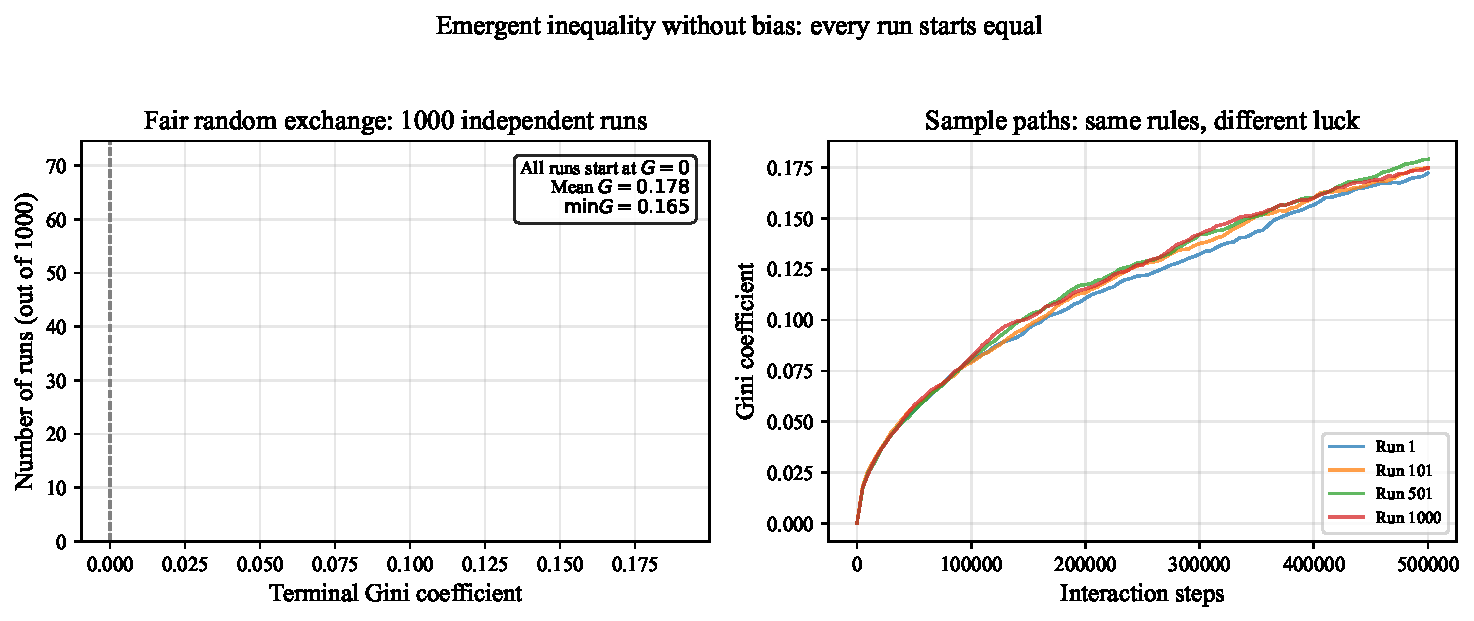
\includegraphics[width=0.98\textwidth]{figures/fig_ensemble_unbiased.pdf}
  \caption{\textbf{Core result.} Left: distribution of terminal Gini across $1{,}000$ unbiased random-exchange runs, each starting from perfect equality. Right: sample Gini paths under the same unbiased rule.}
  \label{fig:ensemble}
\end{figure}

\paragraph{Single-run dynamics.}
Figure~\ref{fig:hist} shows wealth histograms for Model~1 at three time points: a spike at $w=1$ gives way to a spread distribution with no change in agent characteristics.
Figure~\ref{fig:gini} plots Gini over time for all models; the unbiased DY curve (bold) rises monotonically from zero despite fair coins.

\begin{figure}[htbp]
  \centering
  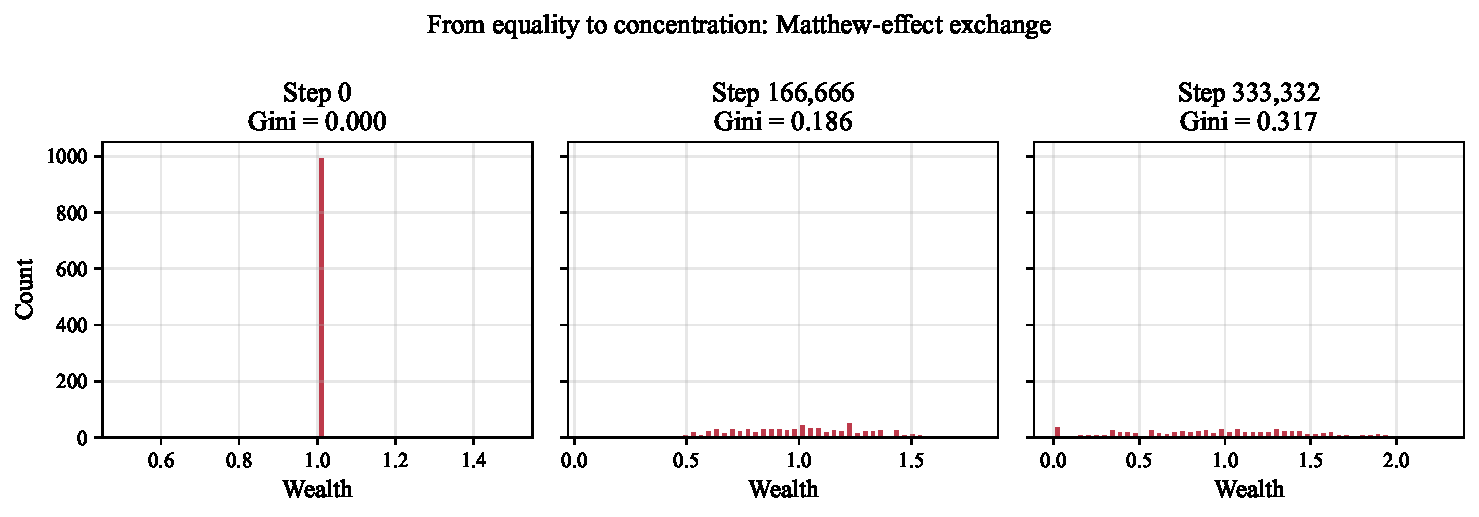
\includegraphics[width=0.95\textwidth]{figures/fig_histogram_evolution.pdf}
  \caption{Wealth histograms under \emph{unbiased} random exchange at three time points.}
  \label{fig:hist}
\end{figure}

\begin{figure}[htbp]
  \centering
  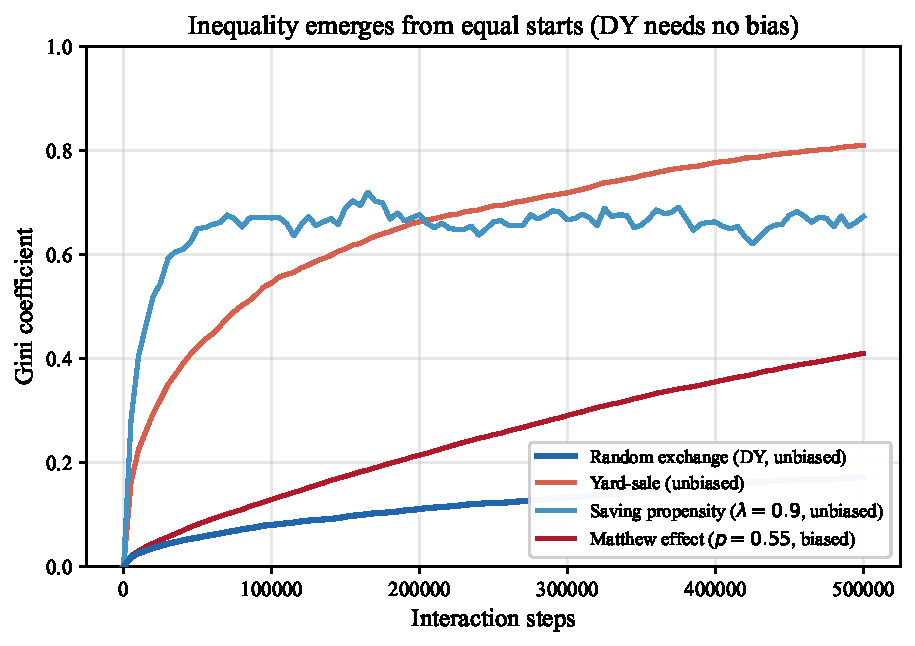
\includegraphics[width=0.92\textwidth]{figures/fig_gini_evolution.pdf}
  \caption{Gini evolution from identical starts. Unbiased DY (bold) requires no Matthew-style bias.}
  \label{fig:gini}
\end{figure}

\paragraph{Stronger dispersion from exchange structure (still unbiased).}
Table~\ref{tab:unbiased} summarizes terminal statistics for Models 1--3.
Yard-sale and saving-propensity rules produce far higher Gini than fair fixed-stake exchange, yet none tilts encounters toward the already-wealthy.

\begin{table}[htbp]
  \centering
  \caption{Unbiased models: terminal inequality ($N=1000$, $5\times 10^5$ steps, seed 42)}
  \label{tab:unbiased}
  \begin{tabular}{lcccc}
    \toprule
    Model & Gini & Top 1\% & Top 10\% & Max / Median \\
    \midrule
    Random exchange (DY)       & 0.17 & 0.02 & 0.15 & 1.9 \\
    Saving ($\lambda=0.9$)     & 0.67 & 0.16 & 0.52 & 68.7 \\
    Yard-sale ($\beta=0.1$)    & 0.81 & 0.14 & 0.66 & 256.0 \\
    \bottomrule
  \end{tabular}
  \vspace{0.4em}
  \begin{minipage}{\textwidth}
    \small\textit{Note:} All three use fair winner/loser selection or no rich-agent tilt. Inequality is emergent, not imposed.
  \end{minipage}
\end{table}

\begin{figure}[htbp]
  \centering
  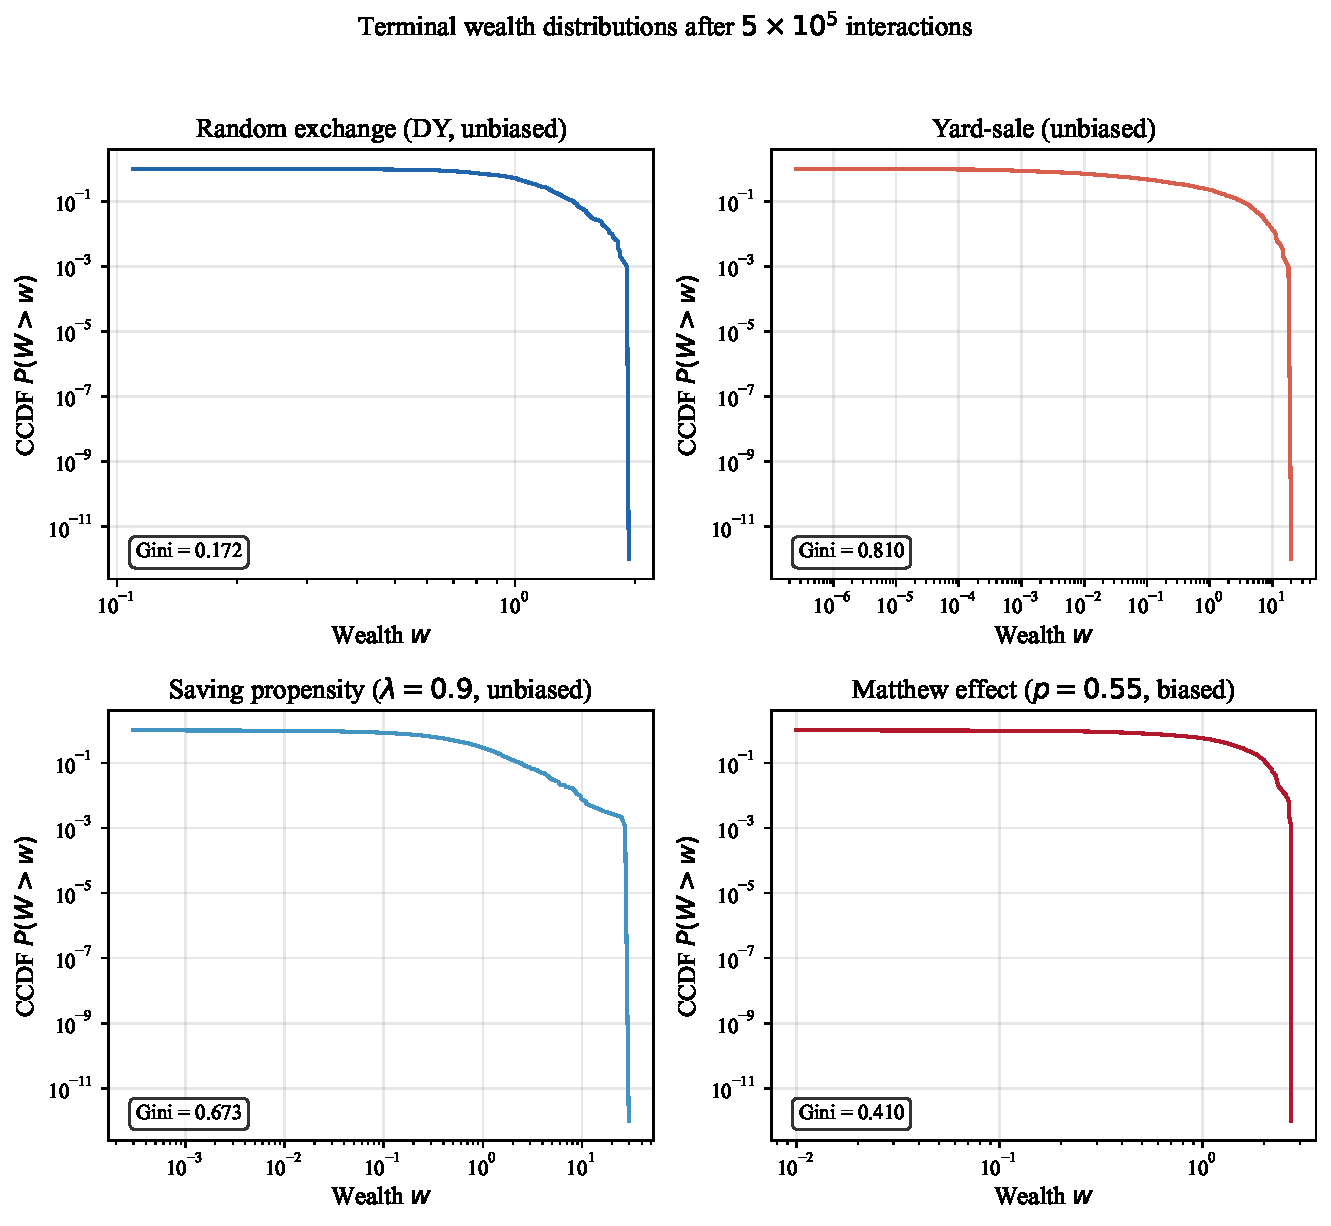
\includegraphics[width=0.95\textwidth]{figures/fig_wealth_distributions.pdf}
  \caption{Terminal wealth distributions (CCDF). Top row: unbiased models.}
  \label{fig:dist}
\end{figure}

\begin{figure}[htbp]
  \centering
  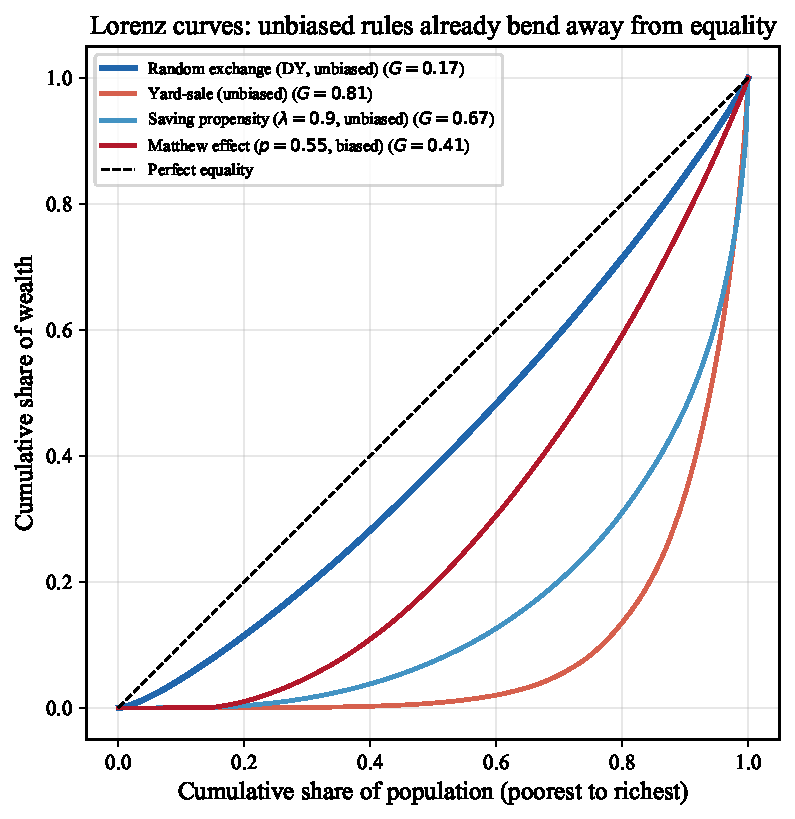
\includegraphics[width=0.65\textwidth]{figures/fig_lorenz.pdf}
  \caption{Lorenz curves. Even unbiased DY bends away from the equality diagonal.}
  \label{fig:lorenz}
\end{figure}

\begin{figure}[htbp]
  \centering
  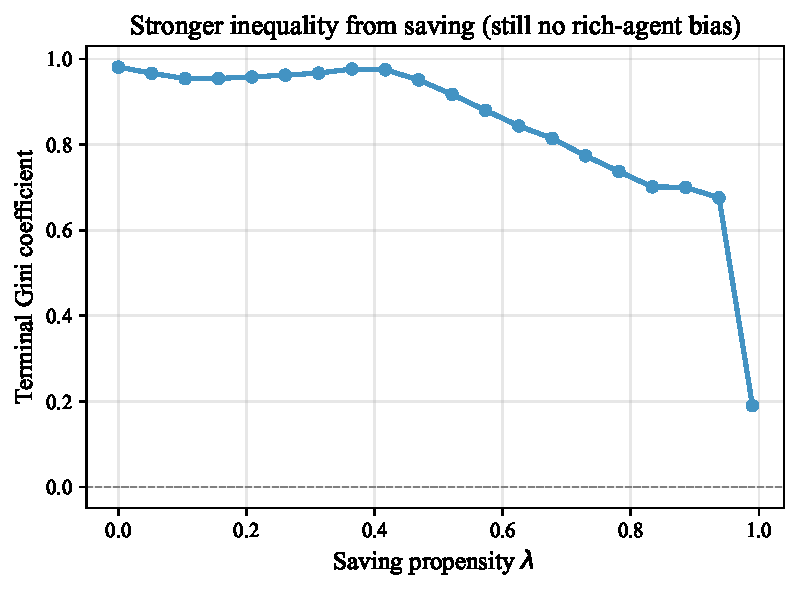
\includegraphics[width=0.72\textwidth]{figures/fig_saving_sweep.pdf}
  \caption{Saving propensity $\lambda$ raises terminal Gini without introducing rich-agent bias.}
  \label{fig:saving}
\end{figure}

% ---------------------------------------------------------------------------
\subsection{Act II: Matthew effect as amplification}
\label{sec:act2}
% ---------------------------------------------------------------------------

\paragraph{Biased exchange accelerates concentration.}
Model~4 does not establish that inequality exists---Act I already did---but asks how much faster it accumulates when encounters favor the richer party.
Figure~\ref{fig:amplification} compares a single unbiased run to $p_{\text{bias}} = 0.55$.
Figure~\ref{fig:ensemble_compare} contrasts the \emph{distribution} of terminal Gini across $500$ runs: Matthew bias shifts mass rightward.

\begin{figure}[htbp]
  \centering
  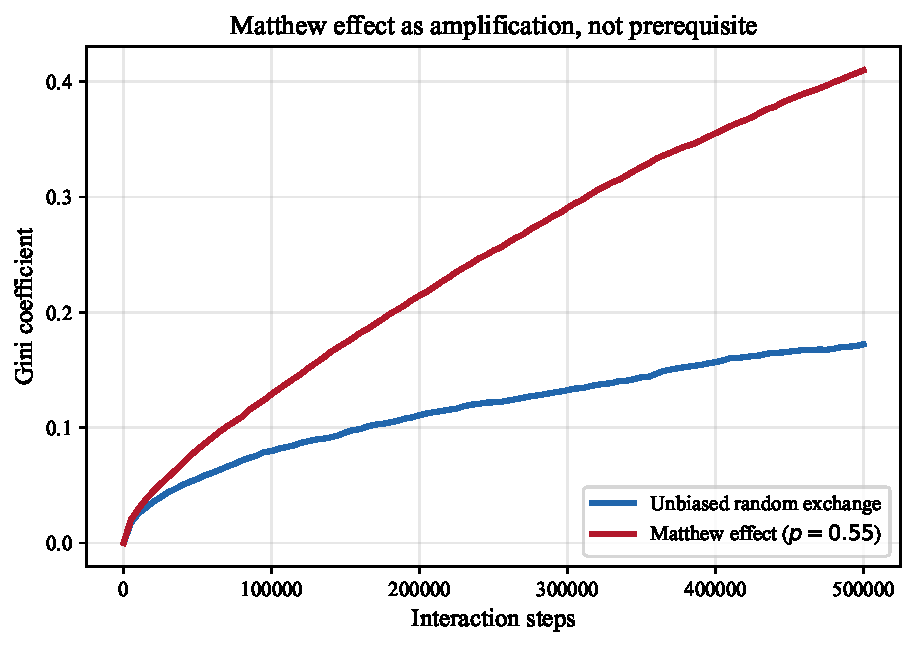
\includegraphics[width=0.92\textwidth]{figures/fig_matthew_amplification.pdf}
  \caption{Matthew effect ($p=0.55$) as amplification of the unbiased baseline.}
  \label{fig:amplification}
\end{figure}

\begin{figure}[htbp]
  \centering
  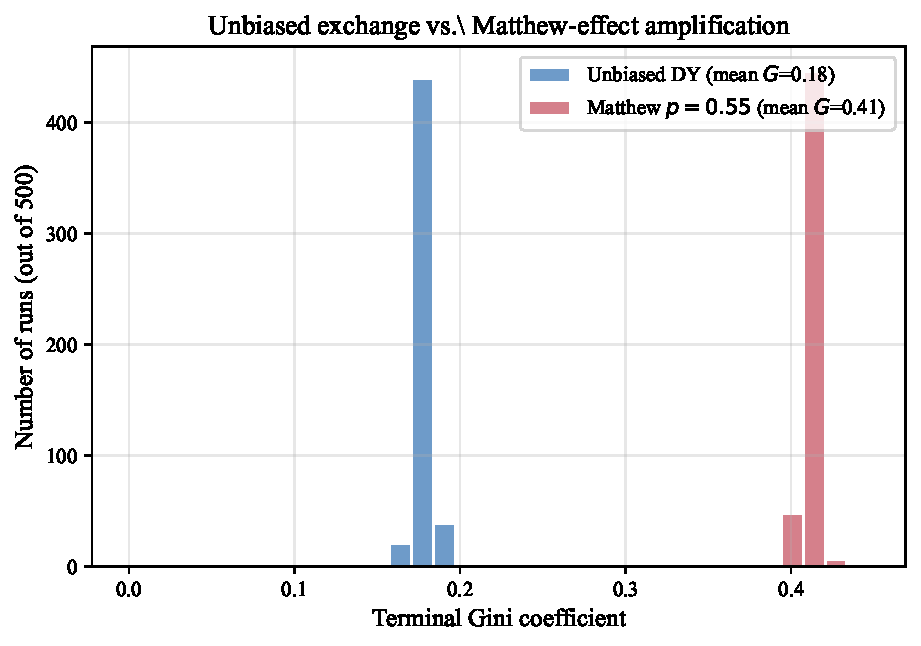
\includegraphics[width=0.88\textwidth]{figures/fig_ensemble_compare.pdf}
  \caption{Terminal Gini across $500$ runs: unbiased DY versus Matthew-effect exchange.}
  \label{fig:ensemble_compare}
\end{figure}

\begin{table}[htbp]
  \centering
  \caption{Extension model: Matthew-effect exchange (seed 42)}
  \label{tab:matthew}
  \begin{tabular}{lcccc}
    \toprule
    Model & Gini & Top 1\% & Top 10\% & Max / Median \\
    \midrule
    Matthew effect ($p=0.55$) & 0.41 & 0.03 & 0.22 & 2.8 \\
    \bottomrule
  \end{tabular}
  \vspace{0.4em}
  \begin{minipage}{\textwidth}
    \small\textit{Note:} Same initial conditions as Table~\ref{tab:unbiased}, but encounters favor the richer agent. Gini exceeds the unbiased DY single-run value ($0.17$) and the DY ensemble mean ($0.18$).
  \end{minipage}
\end{table}

\begin{figure}[htbp]
  \centering
  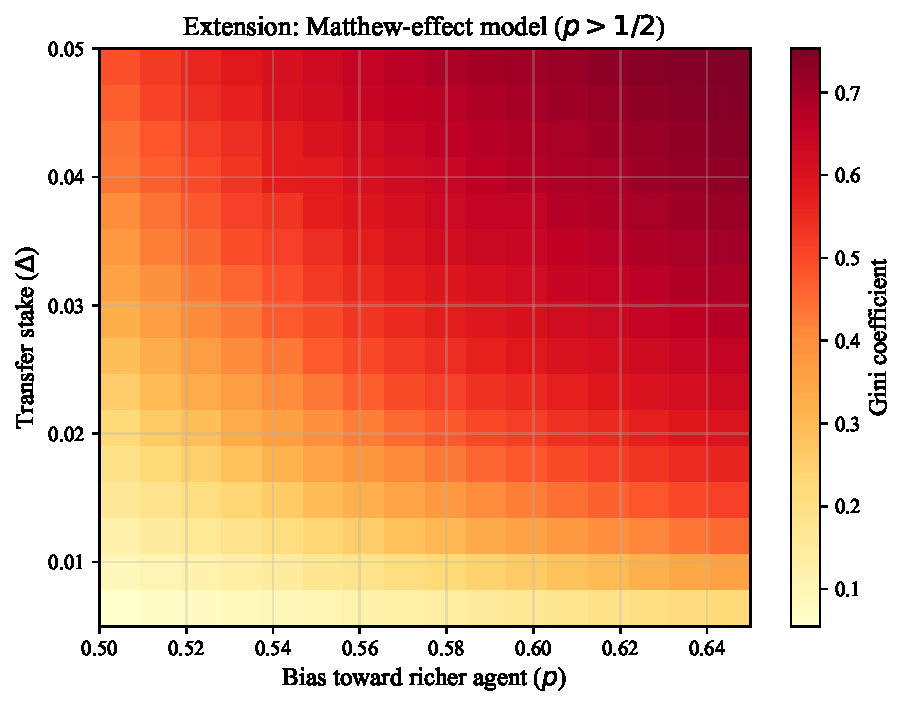
\includegraphics[width=0.75\textwidth]{figures/fig_matthew_heatmap.pdf}
  \caption{Comparative statics in the extension model: terminal Gini vs.\ bias $p$ and stake $\Delta$. At $p=\tfrac{1}{2}$ (dashed), the rule is unbiased.}
  \label{fig:heatmap}
\end{figure}

% ===========================================================================
\section{Discussion}
\label{sec:discussion}
% ===========================================================================

\subsection{Mechanism and intuition}

Three mechanisms operate, in order of generality.

\textbf{First, unbiased random walks.}
Fixed-stake exchange with fair coins is a random walk of wealth with a reflecting boundary at zero.
Variance accumulates even when expected transfers are symmetric \citep{dragulescu2000}.
The $1{,}000$-run ensemble makes the point concretely: every unbiased trajectory leaves perfect equality.

\textbf{Second, multiplicative or min-stake structure.}
Yard-sale and saving rules strengthen tails without rich-agent bias.
The \emph{rules of the bet}, not agent heterogeneity, drive condensation \citep{bouchaud2000}.

\textbf{Third, Matthew-style amplification (extension only).}
A small tilt $p > \tfrac{1}{2}$ accelerates divergence \citep{merton1968, price1976}.
This is cumulative advantage layered on top of the unbiased baseline, not the root cause of dispersion.

For a lay reader: imagine a class where every student starts with \$10 and flips a fair coin each day for \$1.
After many weeks, balances spread apart even though the coin is fair.
That is Act I.
If the coin slightly favors whoever already has more, divergence speeds up.
That is Act II.

\subsection{Relation to empirical inequality and limitations}

Real wealth inequality reflects production, bequests, policy, and heterogeneous returns \citep{piketty2014, benhabib2019, galor2000}.
Our models isolate exchange to prove \emph{existence}: unbiased interaction alone can generate inequality from equality.
The Matthew effect explains \emph{acceleration}, not the bare fact of dispersion.

We caution that simulation comparative statics are internally valid but do not identify real-world institutions.
Finite $N$ and stopping times matter; closed-exchange models omit growth \citep{benhabib2011, acemoglu2015}.

% ===========================================================================
\section{Conclusion}
\label{sec:conclusion}
% ===========================================================================

Identical starting points do not guarantee identical outcomes.
In agent-based wealth-exchange models with conserved aggregate resources, \emph{unbiased} stochastic interaction generates inequality endogenously.
We demonstrate this with $1{,}000$ independent runs of fair random exchange, each beginning at Gini zero and ending with strictly positive dispersion.

The Matthew effect---biasing encounters toward those who already have more---is a meaningful extension that accelerates concentration.
It is not, however, the core explanation for why equality unravels.
The epigraph from Matthew names the amplification mechanism; the primary result is that equality is fragile even without it.

Future work might study ensemble distributions under yard-sale rules, embed agents in networks \citep{dieter2021}, or couple exchange to production and fiscal policy \citep{benhabib2011, piketty2014}.

% ===========================================================================
\bibliographystyle{apalike}
\bibliography{references}

\end{document}
